\chapter{Evaluation}

In this chapter, we aim to present our implemented/adapted motions as a proof of concept. We consider all possible combinations of tasks and ingredients applied to every possible combination of tools and containers. Each task will showcase only one example in this chapter, with the rest available in the appendix. The respective task trees are located in Chapter \nameref{chap:Data_representation}, which illustrates which motions result from combinations of tasks and ingredients.

Through this evaluation, we aim to demonstrate that the knowledge base we have developed can aid in inferring dynamic motions along with parameters that adapt to both the tool and container. Our parameters are relative to the dimensions of the container, specifically the radius within which the motion is executed, as well as the dimensions of the tools used to execute the motion. It is crucial that the motion in the simulation does not exceed the predetermined dimensions, as this could have potentially serious consequences when applied in the real world.
\section{Mixing Task}

\begin{table}[H]
    \centering
    \begin{tabular}{|c|c|c|c|c|}
      \hline
      \textbf{Nr.} & \textbf{Ingredients} & \textbf{Tool} & \textbf{Container} & \textbf{Motion}  \\
      \hline
      1 & Liquid & WoodenSpoon & Salad Bowl & Whirlstorm Motion \\
      \hline
      2 & Dry & WoodenSpoon & Salad Bowl & Whirlstorm Motion \\
      \hline
      3 & Liquid + Dry & WoodenSpoon & Salad Bowl & Whirlstorm Motion \\
      \hline
      4 & Liquid + Wet & WoodenSpoon & Salad Bowl & Whirlstorm Motion \\
      \hline
      5 & Dry + Wet & WoodenSpoon & Salad Bowl & Whirlstorm Motion \\
      \hline
      6 & Wet & WoodenSpoon & Salad Bowl & VerticalCircular + Whirlstorm Motion \\
      \hline
    \end{tabular}
    \caption{Mixing Task}
    \label{tab:mixingtask}
  \end{table}

\begin{itemize}
  \item Inferred Parameters for \textbf{1-5}: 
   \begin{lstlisting}
    => radius_lower_bound_relative = 0.0, 
    radius_upper_bound_relative = 0.7
  \end{lstlisting}
  \item Inferred Parameters for \textbf{6}:
  \begin{lstlisting}
    => radius_lower_bound_relative = 0.0, 
    radius_upper_bound_relative = 0.7,
    vertical_increment = 0.1
  \end{lstlisting}
\end{itemize}

\begin{figure}[H]
  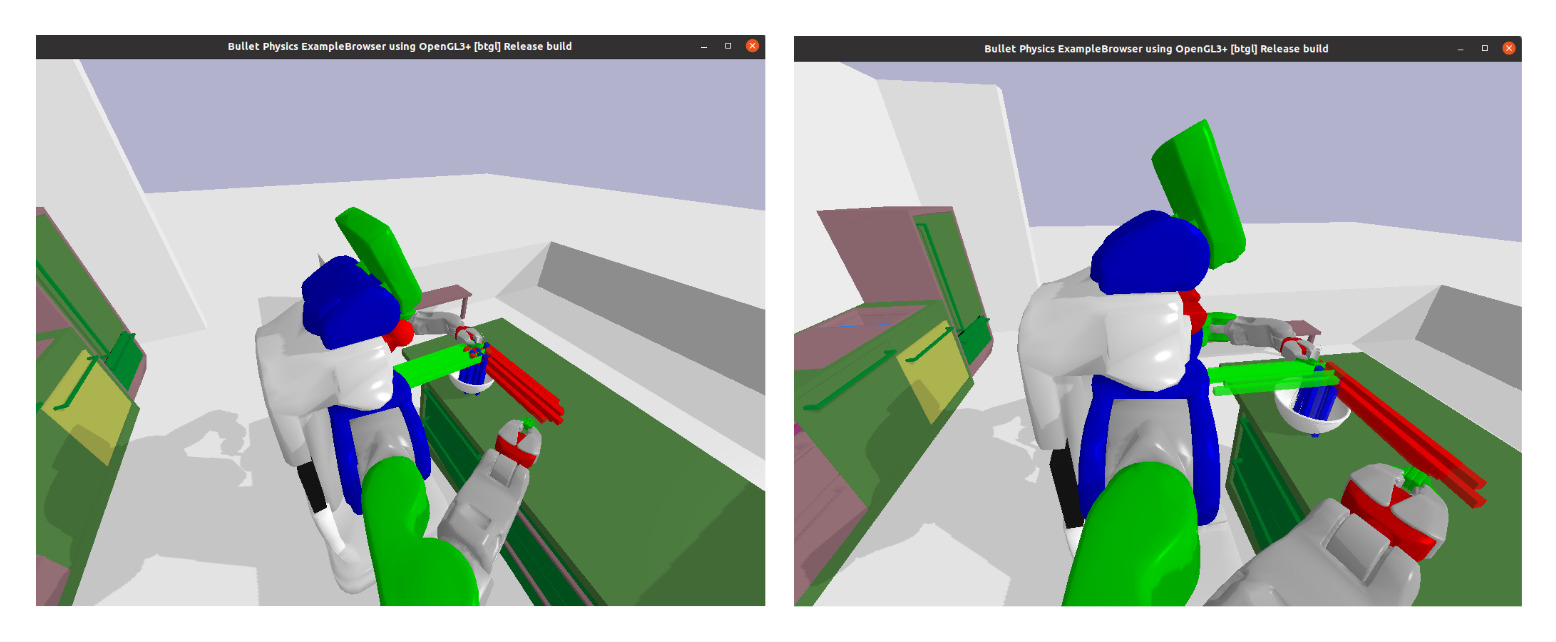
\includegraphics[scale=0.26]{Graphics/mixingtask_rahmen.jpg}
  \caption{Whirlstorm Motion \& Vertical Circular Motion + Whirlstorm Motion}
  \label{fig:mixingverb WikiHow}
\end{figure}

\section{Beating Task}

\section{Stirring Task}

\section{Whisking Task}

\section{Folding Task}